\subsection{Automatyczne kolorowanie czarno-białych obrazów}

  Problem kolorowania czarno-białych obrazów cieszy się dużym zainteresowaniem z
  wielu powodów. Od potrzeb kulturowych takich jak możliwość lepszego
  zwizualizowania oraz zrozumienia przeszłości poprzez kolorowania zdjęć z
  czasów, kiedy występowały one jedynie w kolorach czerni i bieli, po potrzeby
  technologiczne takie jak rekonstrukcja filmów oraz poprawa obrazu cyfrowego.

  Pomimo braku informacji o kolorze w czarno-białych zdjęciach, ludzie są w
  stanie określić potencjalne, rzeczywiste barwy obiektów na zdjęciach bazując
  na treści tych zdjęć oraz swoim doświadczeniu. Można z tego wywnioskować, że
  zdjęcia te zawierają informacje wystarczające do oszacowania potencjalnych
  kolorów. Pozwala to założyć, że do tego zagadnienia można skutecznie wykorzystać
  konwolucyjne sieci neuronowe, które cechują się niezwykłą umiejętnością do
  rozpoznawania wzorców oraz posiadają wyjątkowe zdolności do adaptacji. Z tego
  właśnie powodu sieci splotowe zostaną użyte w przedstawionym rozwiązaniu.

  \subsubsection{Podejście}

  Rozważając możliwe sposoby pokolorowania czarno-białego zdjęcia można spostrzec,
  że kiedy niektóre powierzchnie na zdjęciu mają zazwyczaj oczywiste barwy, niebo
  jest zazwyczaj niebieskie, a trawa zielona, to są też powierzchnie, które
  posiadają szeroki wachlarz możliwych kolorów, na przykład samochodów może być
  zarówno czerwony jak i niebieski albo zielony. Z tego powodu celem zaprezentowanego
  rozwiązania jest niekoniecznie odtworzenie rzeczywistych barw obrazu, a raczej
  wygenerowanie barw, które mogłyby być barwami rzeczywistymi.

  Aby zwiększyć efektywność uczenia wykorzystano przestrzeń barw CIELab. W tej
  przestrzeni barwę obrazu opisują 3 składowe:
  \begin{itemize}
  \item L -jasność (luminacja)
  \item A -barwa od zielonej do magenty
  \item B - barwa od niebieskiej do żółtej
  \end{itemize}
  Przestrzeń barw CIELab została przedstawiona na Rysunku \ref{fig:CIELab}

  \begin{figure}[ht]
    \centering
    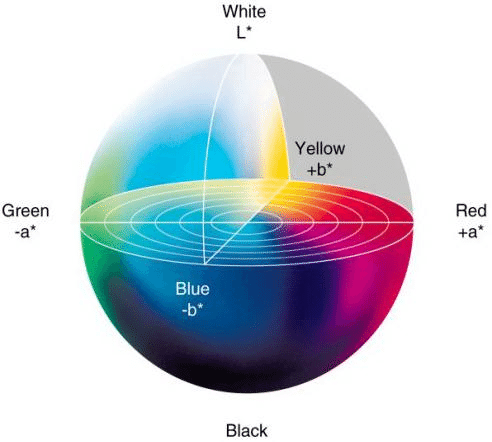
\includegraphics[width=4in]{CIELab}
    \caption[Przestrzeń barw CIELab - źródło:
    \url{https://www.flickr.com/photos/greenmambagreenmamba/4236391637}]
    {Przestrzeń barw CIELab.}
    \label{fig:CIELab}
  \end{figure}

  Zaletą zastosowania CIELab jest fakt, że jest ona najbardziej równomierną
  przestrzenią barw, co oznacza, że jeśli barwy znajdują się w jednakowej
  odległości od siebie w tej przestrzeni, to będą one postrzegane jako jednakowo
  różniące się od siebie. Powinno to zwiększyć skuteczność uczenia sieci oraz
  zapewnić bardziej realistyczne kolorowanie.

  Składowa \textit{L}, jako, że jest identyczna dla obrazu kolorowego jak i
  czarno-białego, stanowi w tym przypadku wejście sieci, na jej podstawie sieć
  odtwarza składowe \textit{A} oraz \textit{B}, które reprezentują przewidziane
  kolory dla obrazu wejściowego.

  Jako rozwiązanie podanej problematyki wpierw został oceniony autorski
  model podstawowy, na jego podstawie zostało przeprowadzone porównanie skuteczności
  różnych konfiguracji, w których uczony był model. Do elementów poddanych
  testom należą algorytm optymalizacyjny, funkcja straty, funkcja aktywacja oraz
  sposób przetwarzania wstępnego danych treningowych.

  \subsubsection{Model podstawowy}

  Opracowany przez nas model jest to FCN. Konwolucyjna część sieci składa się
  z 12 warstw splotowych
  mających na celu nauczyć się mapować składową wejściową \textit{L} na wyjściowe
  składowe \textit{A} i \textit{B}. Składowe wyjściowe muszą mieć takie same
  wymiary jak składowa wejściowe, co oznacza, że kluczowym było odpowiednie dobranie
  parametrów warstw takich jak \textit{padding} (pol. otoczka), \textit{stride}
  (pol. krok) oraz wielkość filtrów. Pełna architektura sieci została przedstawiona w
  Tabeli \ref{table:model_architecture}.
  \noindent\begin{table}[h!]
    \center
    \begin{tabular}{|c | c | m{3.3em} | c | c | m{4em} | c | c| }
     \hline
     Nr & Warstwa & Rozmiar filtra & Stride & Padding & Batch Normalization &
     Fun. aktywacji & Ilość kanałów wej./wyj. \\ [0.5ex]
    \hline
    1 & Splotowa & 3x3 & 1 & 1 & Tak & RELU & 1/32 \\ \hline
    2 & Splotowa & 3x3 & 1 & 1 & Tak & RELU & 32/32 \\ \hline
    3 & Splotowa & 3x3 & 1 & 1 & Tak & RELU & 32/32 \\ \hline
    4 & Splotowa & 3x3 & 1 & 1 & Tak & RELU & 32/32 \\ \hline
    5 & Splotowa & 3x3 & 1 & 1 & Tak & RELU & 32/64 \\ \hline
    6 & Splotowa & 3x3 & 1 & 1 & Tak & RELU & 64/64 \\ \hline
    7 & Splotowa & 3x3 & 1 & 1 & Tak & RELU & 64/64 \\ \hline
    8 & Splotowa & 3x3 & 1 & 1 & Tak & RELU & 64/32 \\ \hline
    9 & Splotowa & 3x3 & 1 & 1 & Tak & RELU & 32/32 \\ \hline
    10 & Splotowa & 1x1 & 1 & 0 & Tak & RELU & 32/32 \\ \hline
    11 & Splotowa & 1x1 & 1 & 0 & Tak & RELU & 32/32 \\ \hline
    12 & Splotowa & 1x1 & 1 & 0 & Nie & - & 32/2 \\ \hline
    \end{tabular}
    \caption{Architektura modelu podstawowego.}
    \label{table:model_architecture}
  \end{table}
  Pierwsza warstwa konwolucyjna rozkłada wejściowy kanał na 32 kanały, co
  pozwala wyciągnąć z niego jak najwięcej informacji o cechach obrazu. Warstwa
  ta ma wielkość filtra 3x3, tak więc aby zachować wymiar kanałów zostały
  zastosowane parametry $\textit{padding}=1$ oraz $\textit{stride}=1$.

  Kolejne trzy warstwy ekstraktują z wejściowych 32 kanałów najbardziej istotne
  cechy związane z powiązaniem treści obrazu z szacowanym kolorem jego powierzchni.
  Warstwy te na swoje wyjście przekazują po 32 kanały zawierające wykryte
  powiązanie pomiędzy pikselami kanałów wejściowych.

  Warstwa piąta rozciąga wejściowe 32 kanały na 64 kanały, dzięki temu kolejne
  2 warstwy przyjmujące na wejście te 64 kanały i przekazujące je na wyjście są
  w stanie wydobyć z obrazu cechy o większym poziomie abstrakcji, co znacznie
  zwiększa skuteczność działania sieci.

  Warstwa ósma ogranicza ilość kanałów w sieci z 64 do 32 wyciągając z nich
  cechy najbardziej przydatne do rozwiązania danej problematyki. Kanały te są
  następnie ponownie przetwarzane przez warwę z wielkością filtru 3x3, co ma
  służyć agregacji rozłożonych cech w bardziej spójną całość, która może być
  już składana w pożądane wyjście.

  Kolejne dwie warstwy w sieci są to warstwy konwolucyjne o wielkości filtru 1x1,
  odpowiadają one warstwom gęstym i mają na celu przekonwertowanie wartości
  funkcji aktywacji z poprzednich warstw na wartości kolorów odpowiadających
  pikseli w przestrzeni barw CIELab. Ostatnia warstwa, również z filtrem o
  wielkości 1x1 zwija 32 kanały otrzymywane na wejściu do 2 kanałów odpowiadających
  składowym \textit{A} oraz \textit{B}, które stanowią pożądany rezultat działania
  sieci.

  Po wszystkich, oprócz ostatniej, warstwach konwolucyjnych znajdują się dodatkowo
  warstwa BatchNorm oraz warstwa funkcji aktywacji RELU mające na celu
  ustabilizować proces uczenia oraz zwiększyć jego efektywność.

  \subsubsection{BatchNorm}

  Warstwa Batch Normalization została przedstawiona w 2015 roku przez S. Ioeffe
  oraz C. Szegedy jako odpowiedź
  na problem zmieniającej się podczas uczenia dystrybucji wartości wejść
  każdej z warstw sieci \cite{BatchNorm}. Ma ona na celu usprawnić i ustabilizować
  trening sieci poprzez normalizację wartości podawanych na funkcje aktywacji.
  Zmienna dystrybucja tych wartości znacznie spowalnia proces uczenia poprzez
  konieczność używania mniejszych wartości współczynnika uczenia, aby
  przeciwdziałać problemom zanikającego oraz wybuchającego gradientu
  \cite{exploding_vanishing_grad} oraz przez potrzebę przemyślanego inicjowania
  wag sieci w celu zwiększenia prawdopodobieństwa nakierowania modelu na pożądane
  rozwiązania w trakcie procesu uczenia.
  % Może jeszcze opisać co to eksplodujący i zanikający gradient

  Podczas uczenia metodą mini-batch (pol. małych paczek), każda paczka jest
  normalizowana w sposób zapewniający zerową wartość średnią oraz
  równą jedności wariancję na przestrzeni wszystkich kanałów wejściowych.
  Zaletą takiego podejścia jest poprawienie przepływu korygującego gradientu
  przez kolejne warstwy sieci podczas fazy wstecznej propagacji błędu. Ponadto
  warstwy BatchNorm zapewniają większą odporność sieci na niekorzystnie zainicjowane
  wagi początkowe modelu.

  Użycie tych warstw w modelu podstawowym tuż za warstwami RELU pozwoliło
  uzyskać bardziej korzystną zbieżność modelu oraz lepsze rezultaty końcowe.
  Ocenione zostało też rozwiązania, w którym warstwy BatchNorm znajdują się
  przed warstwami funkcji aktywacji, lecz dało ono gorsze rezultaty, niż
  podejście wspomniane jako pierwsze.

  \subsubsection{Dropout}

  W trakcie pracy nad ostatecznym modelem podstawowym sprawdzona została
  skuteczność zastosowania warstw Dropout \cite{dropout}. Warstwy te w trakcie
  treningu dezaktywują część neuron aby przeciwdziałać efektowi przeuczania
  się sieci oraz zapewniać wydajny sposób łączenia wielu różnych architektur
  sieci stworzonych do jednego celu w jednolitą całość o skuteczności większej
  niż poszczególne sieci osobno.

  Wybór neuronów, dla których w danej iteracji treningu nie zostaną
  zaktualizowane wagi odbywa się z pewnym prawdopodobieństwem określonym
  podczas inicjalizacji modelu. Dezaktywowanie neuronów można interpretować jak
  przerywanie tymczasowo wszystkich połączeń danego neuronu, zarówno wejściowych
  jak i wyjściowych. Takie działania są równoznaczne z wyselekcjonowaniem z modelu
  mniejszej sieci i trenowaniu wyłącznie jej w aktualnej iteracji. Wagi tej
  podsieci są wtedy współdzielone z modelem źródłowym.
  Jako rezultat uzyskuje się model o znacznie ulepszonych zdolnościach generalizacji.

  Zastosowanie tych warstw w modelu nie przyniosło wyraźnego polepszenia rezultatów
  sieci. W przypadku danej problematyki oraz obranego podejścia do jej rozwiązania,
  przeuczenie sieci nie stanowi wyraźnego zagrożenia, a zastosowanie Dropout
  wiąże się z utratą części informacji kluczowych do odpowiedniego
  generowanie kolorów dla wejściowych obrazów. Model powinien nauczyć się jak
  największej różnorodności kolorów, a Dropout przeciwdziała uczeniu się
  nadmiernej ilości cech przez sieć, co wpływa niekorzystnie na otrzymywane
  rezultaty końcowe. Podczas testów skuteczności tych warstw zostały one umieszczone
  za warstwami BatchNorm. Wizualizacja skutków tej decyzji wraz z rozważeniem
  pozostałych czynników wpływających na efektywność sieci znajduje się w
  sekcji związanej z rezultatami modelu podstawowego.

  \subsubsection{Modyfikacja rozdzielczości}

  W modelach FCN powszechnie stosuje się różne metody zmiany rozdzielczości
  kanałów przechodzących przez sieć, najczęściej są do operacje poolingu mające
  na celu zredukować przestrzenną wielkość reprezentacji cech wyciągniętych z
  obrazu poprzez wyciągnięcie najbardziej istotnych wartości funkcji aktywacji z
  określonych obszarów reprezentacji w celu zredukowania rozmiaru
  sieci, a co za tym idzie, zmniejszenia ilości obliczeń koniecznych do wykonania
  przez sieć.

  Ponadto pooling wspomaga adaptację modelu do zmiennego położenia
  kluczowych wzorów rozpoznawanych przez sieć na obrazie wejściowym. Cecha ta
  zwana jest niezmiennością od translacji (ang. transaltion invariance). Jest
  ona rezultatem dokonywania operacji, takich jak wyliczanie wartości maksymalnej
  z poszczególnych obszarów, dzięki którym zmienne położenie wartości
  selekcjonowanej, a co tym idzie, zmienne położenie ekstraktowanej cechy w obrębie
  danego obszaru nie wpływa na końcową postać reprezentacji przestrzennej obrazu
  wejściowego po przejściu przez warstwę poolingu. Przykładowe operacja poolingu
  została przedstawiona na Rysunku \ref{fig:pooling}.

  \begin{figure}[h]
   \centering
   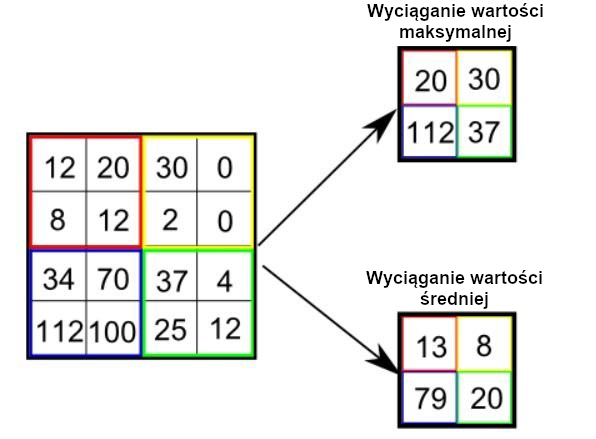
\includegraphics[width=4in]{pooling}
   \caption[Przykładowe operacje warstwy poolingu - źródło: Rysunek własny]{Przykładowe operacje warstwy poolingu}
   \label{fig:pooling}
  \end{figure}

  W modelu końcowym warstwy poolingu nie zostały zastosowane, aby uniknąć utraty
  kluczowych informacji przestrzennych koniecznych to właściwego wygenerowanie
  możliwych barw obrazu.

  \subsubsection{Wykorzystywany zbiór treningowy}

  Do uczenia modelu został wykorzystany zbiór danych CIFAR-10 stworzony przez
  A. Krizhevsky oraz zaprezentowany w 2009 roku \cite{cifar-10}.
  Składa się on z 60000 obrazów w przestrzeni kolorów RGB o rozdzielczości 32 x 32 piksele.
  Spośród tych obrazów 10000 z nich zostało wykorzystanych jako zbiór
  walidacyjny do śledzenia skuteczności treningu modelu. Przykładowe obrazy
  ze zbioru danych zostały przedstawione na Rysunku \ref{fig:cifar10}.

  \begin{figure}[h]
   \centering
   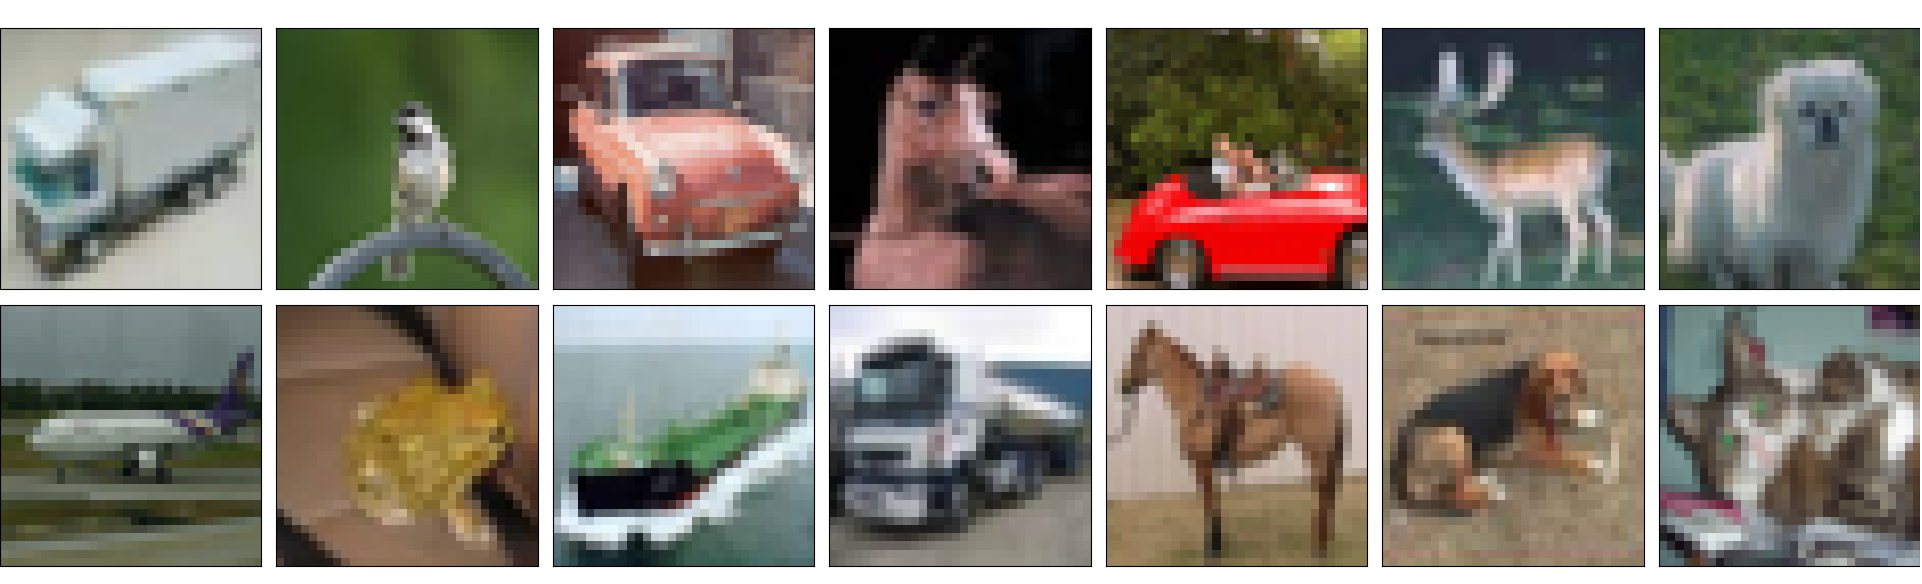
\includegraphics[width=4in]{cifar10}
   \caption[Przykładowe obrazy z CIFAR-10 - źródło: Rysunek własny]
   {Przykładowe obrazy z CIFAR-10}
   \label{fig:cifar10}
  \end{figure}

  Zaletą CIFAR-10 jest niewielka rozdzielczość obrazów co pozwala na mniej
  złożony model oraz szybszy proces uczenia, który można skutecznie przeprowadzić
  nawet przy ograniczonych możliwościach obliczeniowych. Ponadto zbiór ten składa
  się z obrazów dzielących się na 10 klas, tak mała różnorodność klas, a co za
  tym idzie, stosunkowo niewielka ilość możliwych obiektów pojawiających się
  na zdjęciach powinna ułatwić sieci wyuczenie się właściwych barw dla
  identyfikowanych powierzchni. Z drugiej strony mała ilość klas może niekorzystnie
  wpłynąć na umiejętność generalizacji modelu, jednakże obrazy z CIFAR-10
  przedstawiają zróżnicowane otoczenia zawierające obiekty nie kwalifikujące
  się do żadnej klasy, co powinno umożliwić wyuczenia się generalizacji przez
  sieć.

  \subsubsection{Przetwarzanie wstępne danych}

  Przed podaniem na wejście sieci obrazy uczące były wpierw poddawane
  przetwarzaniu wstępnemu mającemu na celu doprowadzić do szybszego oraz
  stabilniejszego treningu modelu. Przetwarzanie wstępne jest kluczowe, gdyż
  wartości o jakie aktualizowane są wagi neuronu zależą w dużej mierze od
  wartości wejść tego neuronu. W przypadku gdy przedziały wartości tych wejść
  nie są jednolite, to może wystąpić duża różnica w tempie aktualizacji wag
  sieci, niektóre wagi będą zmieniane o wiele szybciej niż inne co może spowodować
  destabilizację treningu. Przeskalowanie wszystkich wartości wejściowych do jednakowych
  przedziałów, o niewielkiej wartości maksymalnej i minimalnej oraz wartości
  średniej zbliżonej do zera zmniejsza możliwość wystąpienia tego problemu
  oraz sprzyja ujednoliceniu tempa uczenia się przez sieć rozpoznawania różnych cech.
  Ponadto brak przeskalowania wejść może doprowadzić do zjawisk wybuchającego
  oraz zanikającego gradientu.

  % Przeskalowanie wszystkich wartości wejściowych do jednakowych
  % przedziałów, o niewielkiej wartości maksymalnej i minimalnej oraz wartości
  % średniej zbliżonej do zera, sprzyja ujednoliceniu tempa uczenia się przez sieć
  % rozpoznawania różnych cech.

  W ramach badania rozwiązania przetestowane zostały różne metody przetwarzania
  wstępnego:
  \begin{itemize}
  \item Normalizacja danych na przestrzeni całego zbioru danych z użyciem wartości
  maksymalnej oraz minimalnej całego zbioru, tak aby wartości pikseli danej składowej
  dla każdego obrazu zawierały się w przedziale od -0.5 do 0.5.
  \item Standaryzacja danych na przestrzeni całego zbioru danych z użyciem wartości
  średniej oraz odchylenia standardowego całego zbioru, tak aby uzyskać wartość
  średnią równą w przybliżeniu zero oraz jednostkowe odchylenie standardowe.
  \item Zastosowanie rozmycia gaussowskiego(ang. Gaussian blur) o różnej
  wielkości filtru Gaussowskiego.
  \item Przepuszczenie składowej przez filtr Gaussa o różnej wielkości filtru.
  \end{itemize}

  Rozmycie gaussowskie, zwane także wygładzaniem gaussowskim (ang. Gaussian smoothing),
  jest to operacja polegająca na modyfikacji obrazu z użyciem filtru Gaussa.
  Stosuje się je w celu rozmycia detali na przetwarzanym obrazie, a także by
  ograniczyć ilość występujących na nim zakłóceń oraz szumów. Jest ono powszechnie
  stosowane w fazie przetwarzania wstępnego danych graficznych. W praktyce
  operacja ta sprowadza się do dokonywania splotu kolejnych fragmentów obrazu
  z funkcją Gaussa. Zastosowanie jej na danych wejściowych miało na celu
  zmniejszenie znaczenie detali na obrazie oraz ułatwienie sieci nauczenia się
  rozróżniania rozmaitych powierzchni oraz wzorców.

  Wymienione metody przetwarzania były stosowane w różnych połączeniach oraz
  konfiguracjach zarówno na składowej \textit{L}, jak i składowych \textit{A}
  oraz \textit{B}.


  \subsubsection{Augmentacja danych}



  \subsubsection{Funkcje kosztów}
  % Bez teorii

  \subsubsection{Funkcje aktywacji}

  \subsubsection{Algorytmy optymalizacyjne}
  % Bez teorii

  \subsubsection{Trening}

  \subsubsection{Rezultaty}
